\documentclass[10pt,a4paper]{article}
\usepackage[margin=0.7in]{geometry}
\usepackage{multicol}
\usepackage{amsmath}
\usepackage{tikz}
\usepackage{enumitem}
\usepackage{titlesec}
\usepackage{booktabs}
\usepackage{fontspec}
\usepackage{xcolor}

% Compact formatting
\setlength{\columnsep}{0.7cm}
\setlength{\parindent}{0pt}
\setlength{\parskip}{0.12cm}
\titlespacing{\section}{0pt}{0.4cm}{0.15cm}
\titlespacing{\subsection}{0pt}{0.25cm}{0.08cm}
\titlespacing{\subsubsection}{0pt}{0.2cm}{0.05cm}

% Custom section style
\titleformat{\section}{\large\bfseries}{}{0em}{}
\titleformat{\subsection}{\normalsize\bfseries}{}{0em}{}
\titleformat{\subsubsection}{\normalsize\bfseries\itshape}{}{0em}{}

\begin{document}

\begin{center}
{\LARGE \textbf{Demand, Supply \& Market Equilibrium}}\\[0.15cm]
{\normalsize \textit{Topic 2: The Price Mechanism and Resource Allocation}}\\[0.15cm]
\hrule
\end{center}
\vspace{-0.3cm}

\begin{multicols}{2}
\footnotesize

% ============================================================================
% PART 1: DEFINITIONS AND FOUNDATIONS
% ============================================================================
\section*{1. Core Definitions}

\subsection*{Demand (Detailed)}
\textbf{Demand} is not merely desire; it is \textbf{effective demand} -- the quantity of a good or service that consumers are both \textit{willing} and \textit{financially able} to purchase at each possible price during a specific time period, holding all other factors constant (\textit{ceteris paribus}).

\textbf{Key Elements:}
\begin{itemize}[leftmargin=*,nosep]
    \item \textbf{Willingness:} Derived from utility/preference.
    \item \textbf{Ability:} Backed by purchasing power (income).
    \item \textbf{Time Dimension:} Flow concept (per day/week/year).
    \item \textbf{Price Range:} A schedule, not a single quantity.
\end{itemize}

\textbf{Individual vs. Market Demand:} Market demand is the \textbf{horizontal summation} of all individual demand curves. If consumer A demands 3 units at \$5 and consumer B demands 4 units at \$5, market demand at \$5 is $3+4=7$ units.

\subsection*{Supply (Detailed)}
\textbf{Supply} represents the quantity of a good or service that producers are willing and able to bring to market at each possible price over a given period, \textit{ceteris paribus}.

\textbf{Key Elements:}
\begin{itemize}[leftmargin=*,nosep]
    \item \textbf{Willingness:} Profit motive; price must cover marginal cost.
    \item \textbf{Ability:} Production capacity, technology, resource access.
    \item \textbf{Time Dimension:} Supply elasticity varies with time horizon.
\end{itemize}

% ============================================================================
% PART 2: MEMORY TRIGGERS AND CONCEPTUAL ANCHORS
% ============================================================================
\section*{2. How to Remember (Conceptual Anchors)}

\begin{enumerate}[leftmargin=*,nosep]
    \item \textbf{Demand = Consumer Story:} ``Price high? I buy less.'' (Downward slope). Imagine yourself at a store -- sale prices entice, high prices repel.
    \item \textbf{Supply = Producer Story:} ``Price high? I produce more!'' (Upward slope). Higher price means higher profit margin; firms expand output.
    \item \textbf{Movement vs. Shift -- The ``P'' Test:}
    \begin{itemize}[nosep]
        \item If only \textbf{P} (own price) changes $\to$ \textbf{Movement} along the curve.
        \item If any other factor changes $\to$ \textbf{Shift} of the entire curve.
    \end{itemize}
    \item \textbf{Demand Shifters -- ``PIRATES-CO''}: \textbf{P}opulation, \textbf{I}ncome, \textbf{R}elated goods, \textbf{A}dvertising/Taste, \textbf{T}axes, \textbf{E}xpectations, \textbf{S}eason -- \textbf{C}redit, \textbf{O}ther factors.
    \item \textbf{Supply Shifters -- ``TIC-NES''}: \textbf{T}echnology, \textbf{I}nput costs, \textbf{C}ompeting goods (in production) -- \textbf{N}atural factors, \textbf{E}xpectations, \textbf{S}ellers (number of).
    \item \textbf{Equilibrium = Balance Point}: Imagine a see-saw; the market price is the pivot where the weight of buyers (demand) exactly balances the weight of sellers (supply).
\end{enumerate}

% ============================================================================
% PART 3: MATHEMATICAL FRAMEWORK
% ============================================================================
\section*{3. Mathematical Formulation and Analysis}

\subsection*{Linear Demand Function}
\[
Q_d = a - bP
\]
Where: $a$ = quantity demanded when $P=0$ (intercept), $b$ = slope coefficient (rate at which $Q_d$ changes with $P$). Note: $b > 0$, indicating inverse relationship. \textbf{Inverse Demand:} $P = \frac{a}{b} - \frac{1}{b}Q_d$ (useful for graphing with $P$ on vertical axis).

\subsection*{Linear Supply Function}
\[
Q_s = c + dP
\]
Where: $c$ = quantity supplied when $P=0$ (often negative, as firms need a minimum price to produce), $d$ = slope coefficient ($d > 0$, direct relationship). \textbf{Inverse Supply:} $P = \frac{-c}{d} + \frac{1}{d}Q_s$.

\subsection*{Equilibrium Solution}
At equilibrium, $\mathbf{Q_d = Q_s}$:
\begin{align*}
a - bP &= c + dP \\
a - c &= (b + d)P \\
P^* &= \frac{a - c}{b + d}
\end{align*}
Substituting $P^*$ into either function yields $Q^*$.

\subsection*{Numerical Example}
Given: $Q_d = 80 - 4P$ and $Q_s = -10 + 6P$.
\[
80 - 4P = -10 + 6P \;\Rightarrow\; 90 = 10P \;\Rightarrow\; \mathbf{P^* = 9}
\]
\[
Q^* = 80 - 4(9) = 44 \quad \text{(or } -10 + 6(9) = 44\text{)}
\]

\subsection*{Consumer and Producer Surplus (Advanced)}
\begin{itemize}[leftmargin=*,nosep]
    \item \textbf{Consumer Surplus (CS):} Area below demand curve, above price, up to $Q^*$. $CS = \frac{1}{2} \times Q^* \times (\text{Choke Price} - P^*)$, where choke price = $a/b$.
    \item \textbf{Producer Surplus (PS):} Area above supply curve, below price, up to $Q^*$. $PS = \frac{1}{2} \times Q^* \times (P^* - \text{Min Supply Price})$.
    \item \textbf{Total Welfare:} $CS + PS$; maximized at free-market equilibrium.
\end{itemize}

% ============================================================================
% PART 4: GRAPHICAL ANALYSIS
% ============================================================================
\section*{4. Graphical Analysis}

\subsection*{Basic Market Equilibrium}
\begin{center}
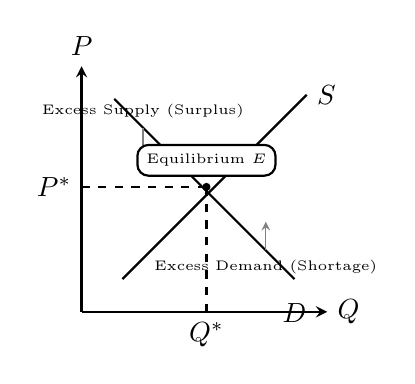
\begin{tikzpicture}[scale=0.52, thick, >=stealth]
    \draw[->] (0,0) -- (6,0) node[right] {$Q$};
    \draw[->] (0,0) -- (0,6) node[above] {$P$};
    \draw[thick] (0.8,5.2) -- (5.2,0.8) node[below=5pt] {$D$};
    \draw[thick] (1,0.8) -- (5.5,5.3) node[right] {$S$};
    \filldraw (3.05,3.05) circle (2pt);
    \draw[dashed] (3.05,0) node[below] {$Q^*$} -- (3.05,3.05);
    \draw[dashed] (0,3.05) node[left] {$P^*$} -- (3.05,3.05);
    % Surplus zone (P > P*)
    \draw[->, thin, gray] (1.5,4.5) node[above, black] {\tiny Excess Supply (Surplus)} -- (1.5,3.8);
    \draw[->, thin, gray] (4.5,1.5) node[below, black] {\tiny Excess Demand (Shortage)} -- (4.5,2.2);
    \node[draw, fill=white, rounded corners] at (3.05,3.7) {\tiny Equilibrium $E$};
\end{tikzpicture}
\end{center}

\subsection*{Panel A: Shift in Demand (Increase)}
\begin{center}
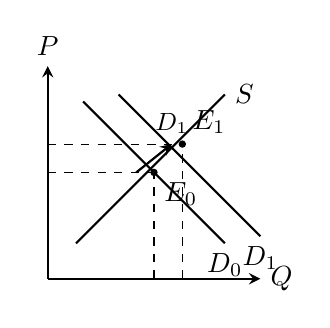
\begin{tikzpicture}[scale=0.45, thick, >=stealth]
    \draw[->] (0,0) -- (6,0) node[right] {$Q$};
    \draw[->] (0,0) -- (0,6) node[above] {$P$};
    \draw (1,5) -- (5,1) node[below] {$D_0$};
    \draw[thick, ->] (2.5,3) -- (3.5,3.8) node[above] {\small $D_1$};
    \draw (2,5.2) -- (6,1.2) node[below] {$D_1$};
    \draw (0.8,1) -- (5,5.2) node[right] {$S$};
    \filldraw (3,3) circle (2pt) node[below right] {$E_0$};
    \filldraw (3.8,3.8) circle (2pt) node[above right] {$E_1$};
    \draw[dashed, thin] (3,0) -- (3,3); \draw[dashed, thin] (3.8,0) -- (3.8,3.8);
    \draw[dashed, thin] (0,3) -- (3,3); \draw[dashed, thin] (0,3.8) -- (3.8,3.8);
\end{tikzpicture}
\end{center}
\textbf{Result:} $P^* \uparrow$, $Q^* \uparrow$. Caused by: income rise, preference surge, price of substitute rises, etc.

\subsection*{Panel B: Shift in Supply (Decrease)}
\begin{center}
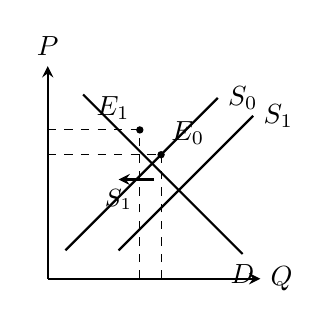
\begin{tikzpicture}[scale=0.45, thick, >=stealth]
    \draw[->] (0,0) -- (6,0) node[right] {$Q$};
    \draw[->] (0,0) -- (0,6) node[above] {$P$};
    \draw (1,5.2) -- (5.5,0.7) node[below] {$D$};
    \draw (0.5,0.8) -- (4.8,5.1) node[right] {$S_0$};
    \draw[thick, ->] (3,2.8) -- (2,2.8) node[below] {\small $S_1$};
    \draw (2,0.8) -- (5.8,4.6) node[right] {$S_1$};
    \filldraw (3.2,3.5) circle (2pt) node[above right] {$E_0$};
    \filldraw (2.6,4.2) circle (2pt) node[above left] {$E_1$};
    \draw[dashed, thin] (3.2,0) -- (3.2,3.5);
    \draw[dashed, thin] (2.6,0) -- (2.6,4.2);
    \draw[dashed, thin] (0,3.5) -- (3.2,3.5);
    \draw[dashed, thin] (0,4.2) -- (2.6,4.2);
\end{tikzpicture}
\end{center}
\textbf{Result:} $P^* \uparrow$, $Q^* \downarrow$. Caused by: input cost rise, natural disaster, tax increase, fewer sellers.

\columnbreak

% ============================================================================
% PART 5: DETERMINANTS (DETAILED EXPLANATIONS)
% ============================================================================
\section*{5. Factors Influencing Demand \& Supply (In-Depth)}

\subsection*{Demand Determinants (Shifters)}
\begin{enumerate}[leftmargin=*,nosep]
    \item \textbf{Income:}
    \begin{itemize}[nosep]
        \item \textbf{Normal Goods:} Income $\uparrow \to$ Demand $\uparrow$ (e.g., branded clothing, restaurant meals). Demand curve shifts \textbf{right}.
        \item \textbf{Inferior Goods:} Income $\uparrow \to$ Demand $\downarrow$ (e.g., instant noodles, public bus transport). Demand curve shifts \textbf{left}.
    \end{itemize}
    \item \textbf{Prices of Related Goods:}
    \begin{itemize}[nosep]
        \item \textbf{Substitutes:} Goods that satisfy similar wants (tea \& coffee). Price of coffee $\uparrow$ $\to$ demand for tea $\uparrow$ (shift right).
        \item \textbf{Complements:} Goods used together (car \& petrol, printer \& ink). Price of car $\uparrow$ $\to$ demand for petrol $\downarrow$ (shift left).
        \item \textbf{Cross-Price Elasticity:} $E_{xy} = \frac{\%\Delta Q_x}{\%\Delta P_y}$. Positive for substitutes, negative for complements.
    \end{itemize}
    \item \textbf{Tastes, Preferences \& Social Trends:} Advertising, celebrity endorsements, cultural shifts, health consciousness (e.g., demand for organic food rising).
    \item \textbf{Consumer Expectations:}
    \begin{itemize}[nosep]
        \item Future price rise expected $\to$ current demand $\uparrow$ (buy now before it's expensive).
        \item Future income rise expected $\to$ current demand $\uparrow$ (spend confidently today).
    \end{itemize}
    \item \textbf{Demographics (Population):} Larger population $\to$ more buyers $\to$ market demand shifts right. Aging population changes composition of demand (more healthcare, less baby products).
    \item \textbf{Government Policies:} Subsidies to consumers (e.g., electric vehicle rebate) shift demand right; taxes on goods (e.g., sugar tax) shift demand left.
    \item \textbf{Seasonal/Climatic Factors:} Demand for ice cream rises in summer, woolen clothes in winter.
    \item \textbf{Availability of Credit:} Easy loans/EMIs $\to$ demand for durable goods (cars, homes) rises.
\end{enumerate}

\subsection*{Supply Determinants (Shifters)}
\begin{enumerate}[leftmargin=*,nosep]
    \item \textbf{Input Prices (Cost of Production):} Wages $\uparrow$, raw material $\uparrow$, energy cost $\uparrow$ $\to$ production cost $\uparrow$ $\to$ supply shifts \textbf{left}. Vice versa.
    \item \textbf{Technology:} Technological progress lowers cost per unit $\to$ supply shifts \textbf{right}. (e.g., automation in manufacturing, AI-driven logistics).
    \item \textbf{Prices of Related Goods in Production:}
    \begin{itemize}[nosep]
        \item \textbf{Substitutes in Production:} A farmer can grow wheat or corn on the same land. Corn price $\uparrow$ $\to$ farmer shifts land to corn $\to$ supply of wheat $\downarrow$ (shift left).
        \item \textbf{Joint Products:} Beef and leather are joint products. Beef demand $\uparrow$ $\to$ leather supply $\uparrow$ (shift right).
    \end{itemize}
    \item \textbf{Producer Expectations:} If firms expect higher future prices, they may withhold current supply (shift left) to sell later at a profit.
    \item \textbf{Number of Sellers (Market Structure):} More firms entering the industry $\to$ market supply shifts \textbf{right}. Exit $\to$ shifts left.
    \item \textbf{Natural/Social Factors:} Weather (drought, flood), pandemics, strikes, war disrupt production $\to$ supply shifts left.
    \item \textbf{Government Policies:}
    \begin{itemize}[nosep]
        \item \textbf{Subsidies:} Reduce effective cost $\to$ supply shifts right.
        \item \textbf{Taxes (Indirect):} Increase cost $\to$ supply shifts left.
        \item \textbf{Regulations:} Environmental/safety compliance costs $\to$ supply shifts left.
    \end{itemize}
\end{enumerate}

% ============================================================================
% PART 6: MARKET EQUILIBRIUM MECHANISM
% ============================================================================
\section*{6. Price Theory: The Market Mechanism}

\subsection*{The Invisible Hand (Adam Smith)}
Prices act as \textbf{signals} in a market economy. When a shortage exists ($Q_d > Q_s$), buyers bid prices up; the higher price incentivizes producers to supply more and discourages some consumption, moving the market toward equilibrium. Conversely, a surplus ($Q_s > Q_d$) leads firms to cut prices, clearing the market. No central planner is needed -- the \textbf{price mechanism} coordinates millions of independent decisions.

\subsection*{Comparative Statics: Effects of Shifts}
\begin{center}
\begin{tabular}{@{}p{1.8cm}p{1.5cm}p{1.2cm}p{1.2cm}@{}}
\toprule
\textbf{Scenario} & \textbf{Shift} & \textbf{$\Delta P^*$} & \textbf{$\Delta Q^*$} \\
\midrule
$D \uparrow$, $S$ constant & $D$ right & $\uparrow$ & $\uparrow$ \\
$D \downarrow$, $S$ constant & $D$ left & $\downarrow$ & $\downarrow$ \\
$S \uparrow$, $D$ constant & $S$ right & $\downarrow$ & $\uparrow$ \\
$S \downarrow$, $D$ constant & $S$ left & $\uparrow$ & $\downarrow$ \\
\addlinespace
$D \uparrow$, $S \uparrow$ (equal) & Both right & \textbf{Same} & $\uparrow$ \\
$D \uparrow$, $S \downarrow$ & $D$ right, $S$ left & $\uparrow$ & \textbf{Ambiguous} \\
$D \downarrow$, $S \uparrow$ & $D$ left, $S$ right & $\downarrow$ & \textbf{Ambiguous} \\
$D \downarrow$, $S \downarrow$ & Both left & \textbf{Ambiguous} & $\downarrow$ \\
\bottomrule
\end{tabular}
\end{center}

\subsection*{Special Cases in Detail}
\begin{enumerate}[leftmargin=*,nosep]
    \item \textbf{Perfectly Inelastic Demand (Vertical $D$):} $E_d = 0$. Quantity demanded fixed regardless of price (e.g., life-saving insulin). Any shift in supply changes only price; quantity remains unchanged. A supply reduction severely raises price without reducing consumption -- a policy concern.
    \item \textbf{Perfectly Elastic Demand (Horizontal $D$):} $E_d = \infty$. Consumers will buy any quantity at exactly one price, but nothing above it (e.g., agricultural commodities in a perfectly competitive global market). A single producer cannot raise price without losing all customers.
    \item \textbf{Government Price Controls:}
    \begin{itemize}[nosep]
        \item \textbf{Price Ceiling} (below $P^*$): Creates persistent \textbf{shortage}. Legal maximum price (e.g., rent control). Quantity supplied falls, quantity demanded rises $\to$ excess demand.
        \item \textbf{Price Floor} (above $P^*$): Creates persistent \textbf{surplus}. Legal minimum price (e.g., agricultural price supports, minimum wage). Quantity supplied exceeds quantity demanded $\to$ excess supply.
    \end{itemize}
    \item \textbf{Veblen Goods (Conspicuous Consumption):} As price rises, snob appeal increases $\to$ demand rises. An \textbf{exception} to the Law of Demand (luxury brands, diamonds).
    \item \textbf{Giffen Goods:} Staple inferior good (e.g., bread in 19th century Ireland). Price rise soaks up so much income that consumers buy more of the staple and less of superior goods (potatoes vs. meat). Extremely rare.
\end{enumerate}

% ============================================================================
% PART 7: EXTENSIVE CASE STUDIES
% ============================================================================
\section*{7. Comprehensive Case Studies}

\subsection*{Case Study 1: The Global Semiconductor Chip Crisis (2020--2023)}

\textbf{Background:} Semiconductors are essential inputs for automobiles, smartphones, medical devices, and virtually all modern electronics. The industry is concentrated in Taiwan (TSMC), South Korea (Samsung), and a few other players.

\textbf{Events (Chronological Analysis):}

\textit{Early 2020 -- Demand Shock:} COVID-19 pandemic triggers global lockdowns. Automakers, anticipating a prolonged recession, \textbf{cancel semiconductor orders}. Simultaneously, remote work and online learning surge, causing a massive spike in demand for laptops, tablets, gaming consoles, and cloud computing hardware. \textbf{Demand for chips shifts sharply right} in consumer electronics segment.

\textit{Mid 2020--2021 -- Supply Shock:} Chip fabrication plants (fabs) face COVID-related shutdowns, worker shortages, and logistics bottlenecks. Key raw material (silicon wafers) supply tightens. A major fire at Renesas plant (Japan, March 2021) and drought in Taiwan (water-intensive chip production) further constrain output. \textbf{Supply curve shifts left dramatically.}

\textit{Late 2021--2022 -- Cascading Effects:} Automakers, having cancelled orders, find themselves at the back of the queue when they try to re-order. Chip foundries are running at full capacity fulfilling tech sector contracts. The auto industry, which uses less advanced chips, cannot get supply. \textbf{A double shock:} $D_{\text{overall}}$ right, $S_{\text{overall}}$ left.

\textbf{Economic Analysis Using Demand-Supply Framework:}

\begin{center}
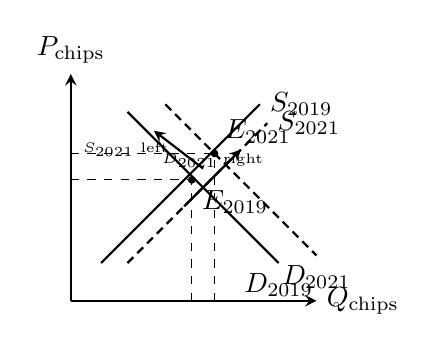
\begin{tikzpicture}[scale=0.48, thick, >=stealth]
    \draw[->] (0,0) -- (6.5,0) node[right] {$Q_{\text{chips}}$};
    \draw[->] (0,0) -- (0,6) node[above] {$P_{\text{chips}}$};
    % Original curves
    \draw (1.5,5) -- (5.5,1) node[below] {$D_{2019}$};
    \draw (0.8,1) -- (5,5.2) node[right] {$S_{2019}$};
    \filldraw (3.2,3.2) circle (2pt) node[below right] {$E_{2019}$};
    % New curves
    \draw[->, thick] (3,2.5) -- (4.5,4) node[midway, above] {\tiny $D_{2021}$ right};
    \draw[thick, densely dashed] (2.5,5.2) -- (6.5,1.2) node[below] {$D_{2021}$};
    \draw[->, thick] (3.5,3.5) -- (2.2,4.5) node[midway, left] {\tiny $S_{2021}$ left};
    \draw[thick, densely dashed] (1.5,1) -- (5.2,4.7) node[right] {$S_{2021}$};
    \filldraw (3.8,3.9) circle (2pt) node[above right] {$E_{2021}$};
    \draw[dashed, thin] (0,3.2) -- (3.2,3.2); \draw[dashed, thin] (0,3.9) -- (3.8,3.9);
    \draw[dashed, thin] (3.2,0) -- (3.2,3.2); \draw[dashed, thin] (3.8,0) -- (3.8,3.9);
\end{tikzpicture}
\end{center}

\textbf{Outcome:}
\begin{itemize}[leftmargin=*,nosep]
    \item \textbf{Price} of semiconductors rose dramatically (spot prices for some chips increased 300--500\%).
    \item \textbf{Quantity} effect was ambiguous in theory, but in practice, severe supply constraints meant overall unit shipments fell slightly despite skyrocketing demand.
    \item \textbf{Automotive Knock-on Effects:} Car production dropped; new car inventory collapsed; used car prices in the US spiked over 40\% year-on-year (a market for a \textit{complement} good affected). Global auto industry lost an estimated \$210 billion in revenue in 2021.
    \item \textbf{Policy Response:} US CHIPS Act (\$52 billion subsidies) aimed to shift \textbf{supply right} long-term by incentivizing domestic fabrication.
\end{itemize}

\textbf{Economic Lessons:}
\begin{enumerate}[leftmargin=*,nosep]
    \item Simultaneous demand increase and supply decrease unambiguously raises price.
    \item Concentrated supply chains create systemic vulnerability.
    \item Government subsidies (supply-side policy) can be justified to address strategic shortages.
    \item Markets are interconnected; a shortage in one input (chips) cascades to final goods (cars, electronics).
\end{enumerate}

\subsection*{Case Study 2: Rent Control in New York City -- A Persistent Price Ceiling}

\textbf{Background:} New York City implemented rent control during World War II (1943 Emergency Price Control Act) to prevent profiteering during a housing shortage. While most US cities abandoned controls, NYC retained \textbf{rent stabilization} covering approximately 1 million apartments today.

\textbf{Mechanism:} The government sets a maximum price (ceiling) below the market equilibrium. Let free-market rent be $P^* = \$2,500/\text{month}$, and rental units available = $Q^* = 500,000$. The city imposes a ceiling at $P_c = \$1,500/\text{month}$.

\textbf{Analyzing the Market:}

At $P_c = \$1,500$:
\begin{itemize}[leftmargin=*,nosep]
    \item \textbf{Quantity Supplied ($Q_s$):} At the artificially low price, landlords have reduced incentive to maintain existing units, construct new rental buildings, or even keep properties in the rental market (conversion to condos/co-ops). $Q_s$ falls to, say, $350,000$ units.
    \item \textbf{Quantity Demanded ($Q_d$):} The lower price makes renting more attractive relative to buying, and more households form (roommates splitting, etc.). $Q_d$ rises to $650,000$ units.
    \item \textbf{Shortage:} Persistent excess demand of $650,000 - 350,000 = 300,000$ units.
\end{itemize}

\begin{center}
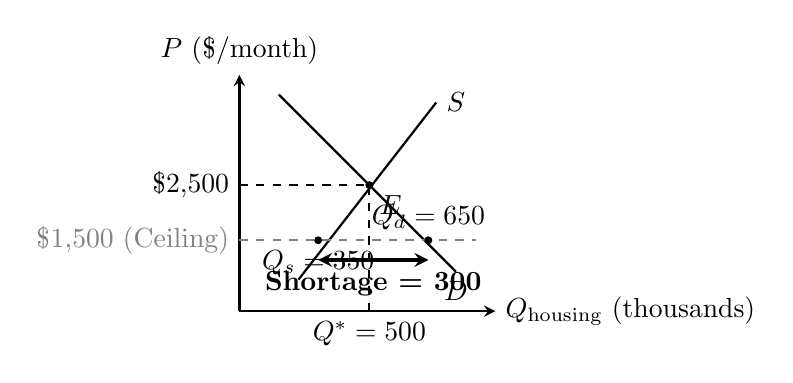
\begin{tikzpicture}[scale=0.5, thick, >=stealth]
    \draw[->] (0,0) -- (6.5,0) node[right] {$Q_{\text{housing}}$ (thousands)};
    \draw[->] (0,0) -- (0,6) node[above] {$P$ (\$/month)};
    \draw (1,5.5) -- (5.5,1) node[below] {$D$};
    \draw (1.5,0.8) -- (5,5.3) node[right] {$S$};
    \filldraw (3.3,3.2) circle (2pt) node[below right] {$E$};
    \draw[dashed, gray, thick] (0,1.8) node[left] {\$1,500 (Ceiling)} -- (6,1.8);
    \filldraw (2,1.8) circle (2pt) node[below] {$Q_s=350$};
    \filldraw (4.8,1.8) circle (2pt) node[above] {$Q_d=650$};
    \draw[<->, very thick] (2,1.3) -- (4.8,1.3) node[midway, below] {\textbf{Shortage = 300}};
    \draw[dashed] (3.3,0) node[below] {$Q^*=500$} -- (3.3,3.2);
    \draw[dashed] (0,3.2) node[left] {\$2,500} -- (3.3,3.2);
\end{tikzpicture}
\end{center}

\textbf{Observed Consequences (Documented by Economists):}

\begin{enumerate}[leftmargin=*,nosep]
    \item \textbf{Misallocation / ``Lock-in'' Effect:} Tenants in rent-controlled units stay for decades, even when the apartment no longer suits their needs (empty nesters in large three-bedrooms), because moving means losing the subsidy. Young families needing space cannot find it. This is \textbf{inefficient allocation} of a scarce resource.
    \item \textbf{Reduced Supply / Deterioration:} Landlords, receiving below-market returns, minimize maintenance (``deferred maintenance''). Buildings deteriorate. Some landlords abandon properties (1960s--70s NYC saw widespread abandonment and arson for insurance). New construction of rental units becomes unprofitable; developers build condos instead.
    \item \textbf{Black Market / Key Money:} Shortage creates illegal side payments. A prospective tenant might pay thousands of dollars ``under the table'' (``key money'') to a departing tenant or broker to secure a rent-controlled lease. The effective price paid (legal rent + key money) approximates the free-market price.
    \item \textbf{Discrimination:} With excess demand, landlords can be highly selective, leading to discrimination based on race, family status, or profession -- because many people compete for each vacancy.
    \item \textbf{Creation of a Dual Market:} A tier emerges: lucky incumbents paying far below market rate, and newcomers paying exorbitant free-market prices for the few available non-controlled units, leading to increased \textbf{inequality}.
    \item \textbf{Economist Consensus:} Surveys show over 90\% of economists agree rent control reduces the quantity and quality of available housing over time. Assar Lindbeck, a prominent economist, famously stated, ``In many cases, rent control appears to be the most efficient technique presently known to destroy a city -- except for bombing.''
\end{enumerate}

\textbf{Economic Lesson:} A binding price ceiling, however well-intentioned, creates a permanent shortage, promotes black markets, reduces quality, and generates deadweight welfare loss. The intended beneficiaries (low-income renters) may suffer from reduced availability and building decay.

% ============================================================================
% PART 8: EXAM QUESTIONS WITH DETAILED ANSWERS
% ============================================================================
\section*{8. Exam Practice Questions \& Model Answers}

\subsection*{Question 1: Analytical}
\textbf{The demand for good X is given by $Q_d = 1200 - 15P$ and supply is $Q_s = 200 + 10P$. The government imposes a per-unit tax of \$5 on producers.}
\textbf{(a) Find pre-tax equilibrium. (b) Find the new supply equation. (c) Calculate post-tax equilibrium price and quantity. (d) Determine tax incidence on consumers and producers. (e) Calculate deadweight loss.}

\vspace{0.1cm}
\textbf{Solution:}
\vspace{0.05cm}
\textbf{(a)} $1200 - 15P = 200 + 10P \Rightarrow 1000 = 25P \Rightarrow \mathbf{P_0^* = 40}$. $Q_0^* = 1200 - 15(40) = \mathbf{600}$.
\vspace{0.05cm}
\textbf{(b)} A \$5 tax on producers means they receive $(P - 5)$ for each unit. Supply function in terms of price received: $Q_s = 200 + 10(P_{\text{received}}) = 200 + 10(P - 5) = 200 + 10P - 50 = \mathbf{150 + 10P}$. New supply: $\mathbf{Q_{s,\text{new}} = 150 + 10P}$.
\vspace{0.05cm}
\textbf{(c)} New equilibrium: $1200 - 15P = 150 + 10P \Rightarrow 1050 = 25P \Rightarrow \mathbf{P_{\text{buyer}} = 42}$. $Q^* = 1200 - 15(42) = \mathbf{570}$. Price received by sellers: $P_{\text{seller}} = 42 - 5 = \mathbf{37}$.
\vspace{0.05cm}
\textbf{(d)} Tax incidence: Consumer pays \$42 (up from \$40, burden = \$2/unit). Producer receives \$37 (down from \$40, burden = \$3/unit). \textbf{Consumer burden: \$2; Producer burden: \$3.} Producers bear more because supply is relatively less elastic ($d=10$) compared to demand ($b=15$). Tax falls more heavily on the less elastic side.
\vspace{0.05cm}
\textbf{(e)} Deadweight loss = $\frac{1}{2} \times \text{Tax} \times \text{Change in Q} = \frac{1}{2} \times 5 \times (600 - 570) = 0.5 \times 5 \times 30 = \mathbf{\$75}$.

\vspace{0.2cm}

\subsection*{Question 2: Conceptual/Discussion}
\textbf{Using the demand-supply framework, explain the likely market effects of a government decision to provide free university education, funded by a tax on high-income earners. Discuss both the education market and potential unintended consequences.}

\vspace{0.1cm}
\textbf{Model Answer:}
Providing free university education is effectively a \textbf{zero price} imposed on students (a price ceiling at \$0) combined with a \textbf{subsidy} to institutions from tax revenue.

\textbf{In the Market for University Seats:}
\begin{itemize}[leftmargin=*,nosep]
    \item \textbf{Demand Side:} Personal cost to attend drops to zero (tuition = 0; though opportunity cost remains). Quantity demanded surges -- many students who would not have attended due to cost now enroll. Demand curve shifts right (or, if modeled as price change, a massive movement down the demand curve).
    \item \textbf{Supply Side:} The government must fund seats through tax revenue, shifting the effective supply curve right if funding is sufficient. However, quantity supplied depends on fiscal capacity. If funding per seat is below true cost, quality may erode.
    \item \textbf{Likely Outcome:} Excess demand (more applicants than funded seats) results in \textbf{non-price rationing} -- admission tests, GPA cutoffs become more competitive. This favors students with better prior schooling (often from higher socioeconomic backgrounds), potentially regressive despite the policy's progressive intent.
\end{itemize}
\textbf{Unintended Consequences:}
\begin{itemize}[leftmargin=*,nosep]
    \item \textbf{Labor Market:} A surge in graduates may depress the wage premium for a degree if demand for skilled labor doesn't keep pace (credential inflation).
    \item \textbf{Opportunity Cost Signal:} Zero tuition removes the price signal that guides students toward fields with high labor demand. Students may choose courses of personal interest over marketable skills, leading to eventual skills mismatch.
    \item \textbf{Tax Burden:} The increased tax on high-income earners may reduce their labor supply, savings, or investment (shift in supply of capital), creating a deadweight loss in other markets.
\end{itemize}
The final welfare effect is ambiguous and depends on the social return to education versus the efficiency cost of taxation.

\vspace{0.2cm}

\subsection*{Question 3: Short Numerical}
\textbf{In the market for coffee, $Q_d = 500 - 2P$ and $Q_s = -100 + 4P$. A technological breakthrough in coffee roasting reduces production cost, shifting supply to $Q_s = 0 + 4P$. Compare the old and new equilibria. Illustrate consumer gain.}

\vspace{0.1cm}
\textbf{Solution:}
\textit{Original:} $500 - 2P = -100 + 4P \Rightarrow 600 = 6P \Rightarrow P = 100, Q = 300$.
\textit{New:} $500 - 2P = 0 + 4P \Rightarrow 500 = 6P \Rightarrow P = 83.33, Q = 333.33$.
\textit{Change:} Price falls by \$16.67; quantity rises by 33.33 units. Consumer surplus increases (area between old and new price, bounded by demand curve). Lower prices benefit all coffee drinkers; producers may earn more total revenue if demand is elastic (here $E_d$ at new point = $|-2 \times 83.33/333.33| \approx 0.5$, inelastic, so TR might fall slightly, but increased volume may raise profit due to lower cost).

\end{multicols}

% ============================================================================
% SINGLE COLUMN SUMMARY TABLE (END OF DOCUMENT)
% ============================================================================
\vspace{0.3cm}
\begin{center}
\fbox{\begin{minipage}{0.9\textwidth}
\footnotesize
\textbf{Summary Table: Cheat Sheet for Exams}
\begin{center}
\begin{tabular}{@{}p{3cm}p{3.5cm}p{3.5cm}@{}}
\toprule
\textbf{Concept} & \textbf{Definition} & \textbf{Key Formula/Effect} \\
\midrule
Law of Demand & Price $\uparrow \to Q_d \downarrow$ & $\frac{\Delta Q_d}{\Delta P} < 0$ \\
Law of Supply & Price $\uparrow \to Q_s \uparrow$ & $\frac{\Delta Q_s}{\Delta P} > 0$ \\
Equilibrium & $Q_d = Q_s$ & $P^* = \frac{a-c}{b+d}$ \\
Movement vs Shift & \textbf{Movement:} Own price change. \textbf{Shift:} Non-price factor change. & Point on same curve vs. new curve. \\
Excess Demand & $Q_d > Q_s$ at given price & Shortage, upward pressure on P \\
Excess Supply & $Q_s > Q_d$ at given price & Surplus, downward pressure on P \\
Price Ceiling & Max price set < $P^*$ & Persistent shortage, black market \\
Price Floor & Min price set > $P^*$ & Persistent surplus, gov't often buys excess \\
Dual Shift Rule & When D \& S both shift & One change (P or Q) always ambiguous \\
\bottomrule
\end{tabular}
\end{center}
\end{minipage}}
\end{center}

\end{document}